\subsection{Overview}

Adversarial 3D objects usually have noisy surfaces to mislead the detection networks.
Thus, surface denoising is needed in the pre-processing unit.
Directly applying the object reconstruction network like IF-Defense\cite{if-defense} will result in high computational overhead and low performance.
Thus, we design a lightweight segmentation algorithm to first crop the potential areas containing obstacles based on laser imaging theory,
and then apply IF-Defense\cite{if-defense} to recover the surface of the 3D object. 

\subsection{Characteristics of adversarial 3D objects}

Adversarial 3D objects are generated by adding, removing, and modifying the 3D points.
These perturbations, however, will always lead to a rough object surface, violating the geometrical features in Figure~\ref{fig:noisy}(b).
When the distance between the vehicle and the adversarial obstacle is larger than the brake distance,
it is easy for the vehicle to mistake this glitchy surface as noise and ignore the overall shape of the obstacle.
In this case, it fails to detect the obstacle and crashes into it.
Therefore, it's important to smooth the noise on the surface and let the out-of-bound points lie on the surface.

\subsection{Recovering methods}

For 3D point clouds, there are broadly two types of methods to recover the distorted surface of 3D adversarial objects.
One is traditional filtering based methods such as VG\cite{VG}, L0\cite{L0}, MLS\cite{mls}. They perform well in removing overall noise in the 3D perception but fail to recover the broken surfaces.
The other is deep neural network based object reconstruction methods such as DUP-Net\cite{dupnet} and IF-Defense\cite{if-defense}.
They aim to recover the broken surface and local part removal attack.

However, they are only evaluated on a single 3D object instead of the outdoor scene perceived by autonomous cars.
It is difficult to apply them directly in AV perception because 1) it will induce large unnecessary computation overhead as the whole road condition is fed as the input, 
and 2) the object reconstruction methods are mostly trained on single object datasets instead of real AV outdoor datasets.

Therefore, in this defense, we first design our own lightweight segmentation algorithm in real AV perception, 
and then apply the latest object reconstruction method - IF-Defense\cite{if-defense}, to remove the noise on the surface.

In the following parts, we first introduce our lightweight segmentation algorithm and then introduce the segmentation-based IF-Defense\cite{if-defense}.

% For 2D images, smoothing can be done with varies filtering methods such as mean filtering\cite{mean-filter} and median filtering\cite{median-filter} 
% and they work quite well.

%% ADD figure 

\begin{figure}
	\centering
	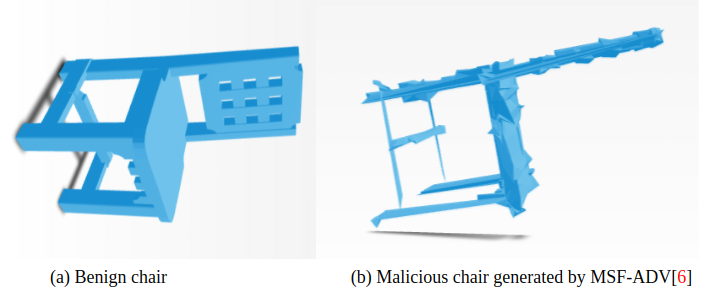
\includegraphics[width=1\linewidth]{figure/benign&ma.png}
	\caption{Benign chair and the malicious version}
	\label{fig:noisy}
\end{figure}

% \begin{figure*}
% 	\centering
% 	\begin{subfigure}{0.5\textwidth}
% 		\centering
% 		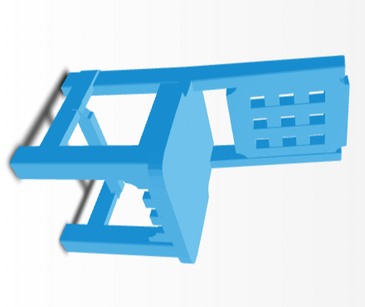
\includegraphics[width=0.6\linewidth]{figure/benign.png}
% 		\caption{Benign chair}
% 		\label{fig:benign}
% 	\end{subfigure}%
% 	\begin{subfigure}{0.5\textwidth}
% 		\centering
% 		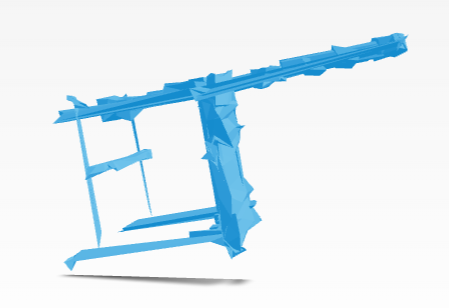
\includegraphics[width=0.7\linewidth]{figure/malicious.png}
% 		\caption{Malicious chair generated by MSF-ADV\cite{msf-adv}}
% 		\label{fig:noisy}
% 	\end{subfigure}
% 	\caption{Water treatment plant architecture and Attack Model}
% 	\label{fig:benign&noisy}
% \end{figure*}

\subsection{Lightweight segmentation algorithm}

Figure~\ref{fig:lidar} is an example of projected LiDAR perception of a traffic cone in the middle of the road. 
These wave-like curves are the result of laser scanning in an open area.
An obstacle will prevent the laser from scanning the area behind it and thus a blank area is formed behind the obstacle.
We can therefore use these white areas to segment the potential areas containing the obstacle.
After that, applying IF-Defense\cite{if-defense} only in these segmented areas will reduce the computation workload.

To segment these areas, we first project the 3D object point cloud with a front view like Figure~\ref{fig:lidar} to get the image of 2D points.
Then we divide the 2D projection into multiple cells illustrated in Figure~\ref{fig:seg}(a).
% How to decide a?
The cell is a square with the edge length \emph{a} to help us calculate the points' distribution. % Add figure
We then calculate the total amount of points in the cell and store it, like in Figure~\ref{fig:seg}(b).
Algorithm~\ref{alg:segment} shows how we get the potential segmentation areas.

% We slide the cell with step \emph{d} horizontallly and vertically from one vertex to another until it walks through every 3D points.

From the observation in Figure~\ref{fig:lidar}, obstacles usually have higher point density followed by a blank shadow-like area. 
Therefore, our goal is to find dense cells which are also accompanied by a series of sparse cells.
First, in Line 7, we sort the array of the number of points in each cell, choose the top \emph{c}\% dense cell numbers as our obstacle set \emph{A} in Line 8, and choose the least \emph{d}\% dense cell as our blank area set \emph{B} in Line 9.
In Line 10, we select one cell \emph{i} from \emph{A}, calculate the Manhattan distance between the \emph{i} and each cell in set \emph{B} according to Eq.~\ref{eq:Manhattan}.

In Eq.~\ref{eq:Manhattan}, $A(i)_x$ represents the $x$ coordinate of $i_{th}$ cell in $A$, i.e., the obstacle set.
 $A(i)_y$ represents the $y$ coordinate of $i_{th}$ cell in $A$.
 $B(i)_x$ represents the $x$ coordinate of $i_{th}$ cell in $B$, i.e., the blank area set.
 $B(i)_y$ represents the $y$ coordinate of $i_{th}$ cell in $B$.
 And the Manhattan distance $d_{ij}$ is the sum of the absolute differences of the coordinates of two points.
We choose this metric because it's fast to calculate and also represents how far two points are from each other. 

Then in Line 15, we sort the array of Manhattan distance $D$ in ascending order.
We further calculate the Manhattan distance among the top \emph{k}\% cells in $D$ in Line 18, to measure the distances among blank area cells. 
In Line 19, we add all the Manhattan distances in $D$ and compare it with a threshold.
If the sum is lower than a threshold \emph{h}, we think these cells are close to each other and might be shadows of the obstacle.
Then we choose the highest and lowest \emph{x} and \emph{y} coordinates of the points and serve this as the segmentation boundary.
Algorithm~\ref{alg:segment} ends when all the obstacles in set A are iterated.
We note that parameters in the algorithm like $c$, $d$, $k$, and $threshold$ have to be decided by experiment and profiling.

\begin{equation}
    \label{eq:Manhattan}
    d_{ij} = |A(i)_x - B(j)_x| + |A(i)_y - B(j)_y|
\end{equation}

\begin{algorithm}[h]
    \caption{Object segmentation algorithm}\label{alg:segment}
    \begin{algorithmic}[1]
    \State $num\_Array$: array of the number of points in each cell
    \State $A$: obstacle sets
    \State $B$: blank area sets
    \State $D$: Manhattan distance array
    \State $sum\_Dis$: Sum of difference in Manhattan distance
    \State $bound\_Dict$: Boundaries of each segmentation
    \State Sort $num_Array$ in descending order
    \State $A$ $\gets$ Top c\% elements in $num_Array$
    \State $B$ $\gets$ Least d\% elements in $num_Array$
    % \State $p\_Array$: final pattern array
    % \State $p\_Dict$: dictionary of detected pattern
    % \State $idx$: the number of elements to match
    % \State $idx \gets 2$ 
    % \State $p \gets arrayofPac[0:1]$
    \While{$A$ is not fully checked}
        \While{$B$ is not fully checked}
            \State $d_{ij}$ = |$A(i)_x$ - $B(j)_x$| + |$A(i)_y$ - $B(j)_y$|
            \State add $d_{ij}$ into $D$
        \EndWhile
        \State Sort $D$ in ascending order
        \State $D$ $\gets$ Top $k$\% $D$

        \While{$D$ is not fully checked}
            \State $diff$ = |$D(i)_x$ - $D(i+1)_x$| + |$D(i)_y$ - $D(i+1)_y$| 
            \State $sum\_Dis$ += $diff$
        \EndWhile
        \If{$sum\_Dis$ < $threshold$}
            \State $bound\_Dict[i]$ $\gets$ smallest $x$ coordinate in $D$
            \State $bound\_Dict[i]$ $\gets$ largest $x$ coordinate in $D$
            \State $bound\_Dict[i]$ $\gets$ smallest $y$ coordinate in $D$
            \State $bound\_Dict[i]$ $\gets$ largest $y$ coordinate in $D$
        \EndIf
    \EndWhile
    \State return $bound\_Dict$
    \end{algorithmic}
    \end{algorithm}

\begin{figure}
	\centering
	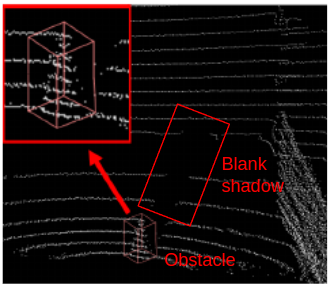
\includegraphics[width=0.5\linewidth]{figure/lidar.png}
	\caption{LiDAR perception. Modified from Figure 10 in \cite{msf-adv}}
	\label{fig:lidar}
\end{figure}

\begin{figure*}
	\centering
	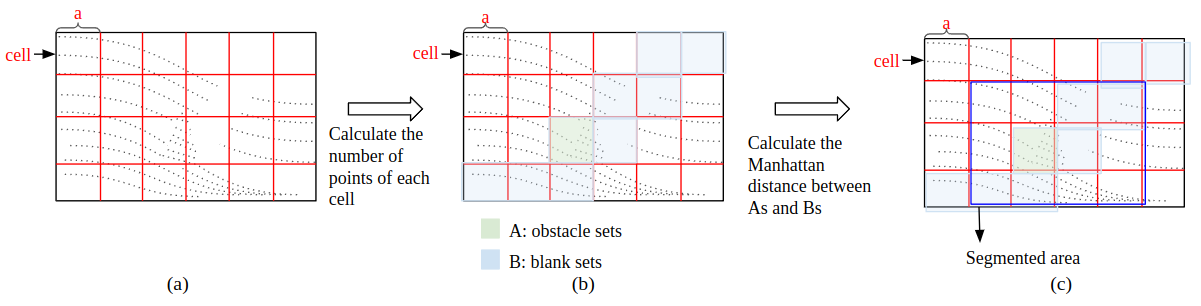
\includegraphics[width=1\linewidth]{figure/segmentation.png}
	\caption{Segmentation algorithm}
	\label{fig:seg}
\end{figure*}



\subsection{Segmentation-based IF-defense} 
IF-defense\cite{if-defense} is a framework to recover the corrupted surface of the point cloud based on the implicit function\cite{implicit}.
It aims to optimize the shape of 3D objects to follow the geometry property and realize the uniform distribution of 3D points.
It uses geometry-aware and distribution-aware loss functions to encourage the optimized points to lie on the surface as well as distribute more evenly.
IF-defense\cite{if-defense} is implemented with ONet\cite{ONet} and ConvONet\cite{ConvONet} network.
However, the dataset that IF-defense\cite{if-defense} uses is ShapeNet\cite{shapenet}, which is a set of single clean 3D objects.
It hasn't been tested on AV scenarios such as the KITTI\cite{kitti} dataset. 

One big challenge of applying it on point clouds in AV outdoor perception is that there are multiple objects existing in the scene, like roads, buildings, vehicles, and pedestrians.
Since we aim at removing the obstacle noises fed into the object detection network, recovering the whole point cloud including the road is a waste of resources.
Also, it may not perform well in AV outdoor perception due to the different training dataset.

Thus, we plan to first use the lightweight segmentation algorithm to get the potential recovery areas.
Then we apply the IF-defense\cite{if-defense} to recover the selected areas.
At last, we replace the originally selected point clouds with the recovered point clouds and feed the combined output into the pre-processing unit in the AV perception module. 
In this way, we hope to recover the LiDAR detection output before sending it to the sensor fusion part.
